\documentclass[11pt]{article}


% TODO: use polyflossia
\usepackage[english, spanish]{babel}

% font specification
\usepackage{fontspec}
% \setmainfont{TeX Gyre Pagella}
% \setmainfont[Mapping=tex-text]{TeX Gyre Pagella}
% \setmainfont[Ligatures=TeX]{TeX Gyre Pagella}

\setmainfont[Mapping=tex-text]{LinLibertineO}
\newfontfamily\ipa{LinLibertineO}

% \setsansfont[Scale=MatchLowercase]{Latin Modern Sans}
% \setsansfont[Scale=MatchLowercase]{Linux Biolinum O}
\setsansfont[Scale=MatchLowercase]{Carlito}

% consolas no es free pero tiene bold, inconsolata es al vesre
% \setmonofont[Scale=MatchLowercase]{Inconsolata}
% \setmonofont[Scale=MatchLowercase]{Consolas}
\setmonofont[Scale=MatchLowercase]{DejaVu Sans Mono}

% page sizes and margins
\usepackage{geometry}
\geometry{paper=a4paper, left=2.75cm, right=2.75cm, bottom=2.5cm, foot=2cm, top=3.5cm}
\setlength{\headheight}{14pt}

% hyperlinks in pdfs
\usepackage{hyperref}
\hypersetup{pdftitle=, pdfauthor=,pdfborder={0 0 0}, colorlinks=false, linkcolor=black, citecolor=black, filecolor=black}
\hypersetup{pdftitle={Resolución de la ecuación de transporte mediante el método de las características en el código neutrónico milonga}, pdfauthor={Ramiro Vignolo}}

% headers & footers
\usepackage{fancyhdr}
\makeatletter
\fancyhead[L]{}
\fancyhead[C]{}
\fancyhead[R]{\thepage/\pageref{lastpage}}
\fancyfoot[L]{}
\fancyfoot[C]{\tiny{\texttt{Asociación Argentina de Tecnología Nuclear}}}
% \fancyfoot[R]{\thepage}
\fancyfoot[R]{}
\makeatother
\renewcommand{\headrulewidth}{0.4pt}
% \renewcommand{\footrulewidth}{0.4pt}
\pagestyle{fancy}

% biblatex
\usepackage{csquotes}     % this package is needed for \blx@bibinit below (sic)
\usepackage[backend=biber,sorting=none]{biblatex}    
\addbibresource{bibliografia/bibliografia.bib}
\addbibresource{bibliografia/congresos.bib}
\addbibresource{bibliografia/informes.bib}
\addbibresource{bibliografia/internacionales.bib}
\addbibresource{bibliografia/monografias.bib}
\addbibresource{bibliografia/nacionales.bib}
% initialize macros so \bibstring can be used to show some fields (needs csquotes)
\makeatletter
\blx@bibinit
\makeatother

% Font style for figures' and tables' captions
\usepackage[small,bf,up]{caption}
\renewcommand{\captionfont}{\scriptsize\sf}

% things
\usepackage{lastpage}
\usepackage{graphicx}
\usepackage{amsmath}
\usepackage{amssymb}
\usepackage{rotating}
\usepackage{tabularx}
\usepackage[table]{xcolor}
\usepackage{eso-pic}
\usepackage{subfig}
\usepackage{listings}
\usepackage{xltxtra}
\usepackage{siunitx}


\usepackage{booktabs}
\usepackage{lscape}
\usepackage{breqn}

% vectors done right
\renewcommand{\vec}[1]{\ensuremath\mathbf{#1}}

% textpos para poner bloques de texto en posiciones absolutas
\usepackage[absolute]{textpos}
\setlength{\TPHorizModule}{2.5mm}
\setlength{\TPVertModule}{\TPHorizModule}
\textblockorigin{0mm}{\paperheight}


\makeatletter 
% these fields are defined as TeX macros so they can be used as such,
% i.e.  in the fancyhdr package
\def\affiliation#1{\def\@affiliation{#1}}

\newcommand{\fielddesc}[1]{\textsf{\footnotesize{#1}}}

\def\maketitle{%
\thispagestyle{empty}

% --- title -------------------------------------------------------
\null
\vspace{0.5cm plus 0.5cm minus 0.5cm}

\begin{center}
\begin{minipage}{0.8\linewidth}
\begin{center}
\Large{\textbf{\textsc{\@title}}}

\vspace{0.75cm plus 0.2cm minus 0.1cm}

\large{\@author}

\vspace{1.25cm plus 0.25cm minus 0.25cm}

\small{\@affiliation}
\vspace{1cm plus 0.2cm minus 0.2cm}

\end{center}
\end{minipage}
\end{center}

}

\makeatother

\begin{document}


\title{Resolución de la ecuación de transporte mediante el método de las características en el código neutrónico milonga}
\author{Vignolo, R.$^{1}$}
\affiliation{%
$^1$TECNA Estudios y Proyectos de Ingeniería S.A.\\
Encarnaci\'on Ezcurra 365, C1107CLA~Buenos Aires, Argentina\\
\url{rvignolo@tecna.com}\\
}


\maketitle


\begin{abstract}
\noindent
Milonga es un código de cálculo neutrónico que resuelve la ecuación de transporte estacionaria y multigrupo tanto mediante la formulación de difusión como la de ordenadas discretas ($S_N$) sobre mallas no estructuradas (aunque mallas simples estructuradas son también soportadas). Ambas formulaciones pueden ser resueltas sobre esquemas de volúmenes o elementos finitos. Milonga nació como parte del desarrollo de una tesis de doctorado de ingeniería nuclear y, al ser \emph{software} libre, permite que distintos colaboradores participen activamente en su desarrollo y no ser, como Stamm'ler decía, usuarios que ``\emph{will never understand the programs they are to use and, as computer slaves, consider them as black boxes, blindy trusting their results''} (Stamm'ler et al., 1983). La implementación del método de las características (MOC) incorpora dentro de milonga una formulación capaz de ser aplicada en cálculos de celda, rellenando la etapa faltante en cálculos de producción: celda (MOC), celda-núcleo ($S_N$) y núcleo (difusión). En esta primera instancia del desarrollo de formulaciones de celda, MOC fue seleccionado por sobre el método de las probabilidades de colisión debido a que éste no produce matrices densas, por lo que es posible resolver problemas con mayor cantidad de regiones. En este contexto, se desarrolló un eficiente algoritmo de \emph{ray tracing} sobre mallas no estructuradas y estructuradas y un \emph{solver} de potencias no lineal que, mediante la resolución de la ecuación de transporte en cada \emph{track}, permite obtener el flujo escalar en cada región y grupo de energía. En este trabajo se discute acerca de la implementación del método, los resultados preliminares obtenidos y las futuras mejoras e incorporaciones.
\end{abstract}

\vfill

\begin{center}
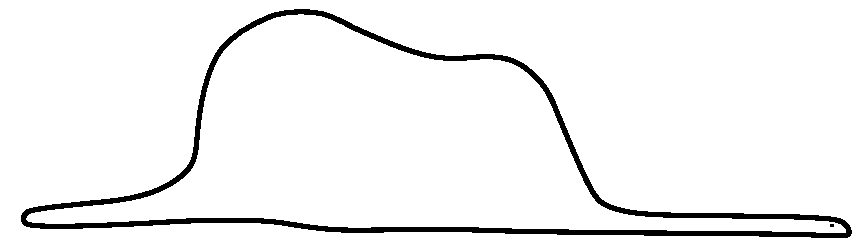
\includegraphics[width=5cm]{vibora-blanca-sola.pdf}
\end{center}

\vfill

\begin{center}
\begin{small}
XLIII Reunión Anual de la Asociación Argentina de Tecnología Nuclear\\
Buenos Aires, Noviembre 2016
\end{small}
\end{center}

\pagebreak

\title{Solving the neutron transport equation by the method of characteristics in milonga neutron code}
\author{Vignolo, R.$^{1}$}
\affiliation{%
$^1$TECNA Estudios y Proyectos de Ingeniería S.A.\\
Encarnaci\'on Ezcurra 365, C1107CLA~Buenos Aires, Argentina\\
\url{rvignolo@tecna.com}\\
}


\maketitle

\selectlanguage{english}
\begin{abstract}
\noindent
Milonga is a neutron code that solves the steady-state multigroup neutron transport equation either by using the diffusion approximation or the discrete ordinates method ($S_N$) over unstructured grids (although simple structured grids can also be used). Both formulations can be solved over a finite-volumes or a finite-elements discretization scheme. Milonga was born as part of a PhD in nuclear engineering and, since it is free software (as in free speech), it may be developed collaboratively by volunteer engineers/computer programmers who do not want to be, as Stamm'ler used to say, users that ``\emph{will never understand the programs they are to use and, as computer slaves, consider them as black boxes, blindy trusting their results''} (Stamm'ler et al., 1983). The implementation of the method of characteristics (MOC) incorporates in milonga a lattice formulation, filling in the missing stage of production calculations: lattice (MOC), lattice-core ($S_N$) and core (diffusion). In this first stage of development of lattice formulations, MOC was selected because it overcome the main limitation for collision probability (CP) method: it does not produce full square matrices of order equal to the number of regions in the domain times the energy groups, so it is possible to solve problems with many more regions. In this context, an efficient ray tracing algorithm for structured and unstructured meshes and a non-linear power method were developed. These two things allow to compute the scalar flux per refion and energy group by collecting all mean angular fluxes over track segments and region sources. This paper discusses about the implementation of the method, preliminary results and future improvements or additions in milonga.
\end{abstract}

\vfill

\begin{center}
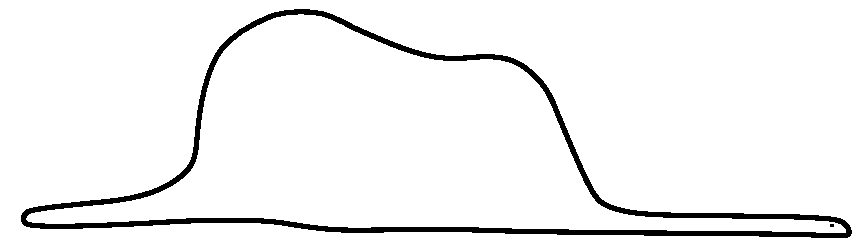
\includegraphics[width=5cm]{vibora-blanca-sola.pdf}
\end{center}

\vfill

\begin{center}
\begin{small}
XLIII Reunión Anual de la Asociación Argentina de Tecnología Nuclear\\
Buenos Aires, November 2016
\end{small}
\end{center}

\addtolength{\textheight}{-2cm}

\pagebreak

\selectlanguage{spanish}

\tableofcontents
\pagebreak


\section{Introducción}

Los cálculos de celda se corresponden, tradicionalmente, con el primer paso del análisis determinístico de reactores. En esta instancia, una celda representativa es resuelta mediante una formulación que pueda ser correctamente aplicada al dominio. Entre estas formulaciones, usualmente se utilizan tanto el método de las probabilidades de colisión (que puede estar asociado al método de las corrientes en las interfaces) como el método de las características. La resolución de la ecuación de transporte en este dominio resulta en la obtención del flujo escalar en una discretización fina en energía y regiones que, posteriormente, es empleada para calcular secciones eficaces homogeneizadas tanto en energía como en el espacio a utilizar como entradas en cálculos de núcleo.

En un comienzo, la celda elemental consistía en un \emph{pin cell} donde sólo se representa una única barra combustible junto al moderador que la rodea y condiciones de contorno reflectivas. Debido al incremento en el poder de cálculo, hoy en día es posible realizar cálculos de celda a nivel de elemento combustible e incluso se busca realizarlos a nivel de núcleo. El método de las características (comúnmente denominado MOC) pareciera ofrecer esta posibilidad, y es por este motivo que durante los últimos años ha ganado un particular interés. 

Milonga es un código neutrónico de núcleo escrito como \emph{plugin} de wasora~\cite{wasora}. Con la incorporación del método de las características como formulación de transporte en 2D se ha abierto el panorama a los cálculos de celda. En este trabajo se describe la implementación de MOC 2D y se presentan algunos resultados preliminares. Por último, se hará un breve hincapié en futuras incorporaciones.


\section{Método de las Características}

MOC resuelve la forma característica de la ecuación de transporte recorriendo lineas rectas (denominadas rayos o \emph{tracks}) que simulan la trayectoria de neutrones a medida que se mueven por el dominio. Este método se basa en la resolución iterativa del flujo a partir de la resolución de la ecuación de transporte sobre dichos \emph{tracks} trazados. El método de las características es generalmente aplicado sobre la forma multigrupo de la ecuación de transporte y sobre dominios compuestos por regiones con propiedades nucleares uniformes. Posteriormente, el flujo escalar de cada región y grupo es computado a partir de la variación del flujo angular sobre cada uno de los \emph{tracks} y de la fuente. 

\subsection{Discretización y nomenclatura}

Debido a la gran cantidad de notación disponible en la bibliografía, es conveniente definir adecuadamente la discretización a utilizar en este trabajo previo a ingresar a la descripción del método. Las diferentes definiciones que se dan a continuación se encuentran representadas gráficamente en la figura~\ref{fig:coords-indices}. En este contexto, se definen:

\begin{itemize}
\renewcommand\labelitemi{$\cdot$}
 \item $g$: índice asociado a un grupo de energía;
 \item $i$: índice asociado a una región con flujo plano;
 \item $m$: índice asociado a un ángulo s\'olido $\boldsymbol{\hat{\Omega}}_m$ (cada índice $m$ tiene asociado un único par de índices $a$ y $p$, que son detallados a continuación);
 \item $a$: índice asociado a un ángulo azimutal $\varphi_a$;
 \item $p$: índice asociado a un ángulo polar $\theta_p$; y
 \item $k$: índice asociado a un segmento de un \emph{track}; $k$ generalmente viene acompañado de los índices $i$ y $m$ para representar los segmentos contenidos en la región $i$ con ángulo $\boldsymbol{\hat{\Omega}}_m$.
\end{itemize}

\begin{figure}[!h]
 \begin{center}
  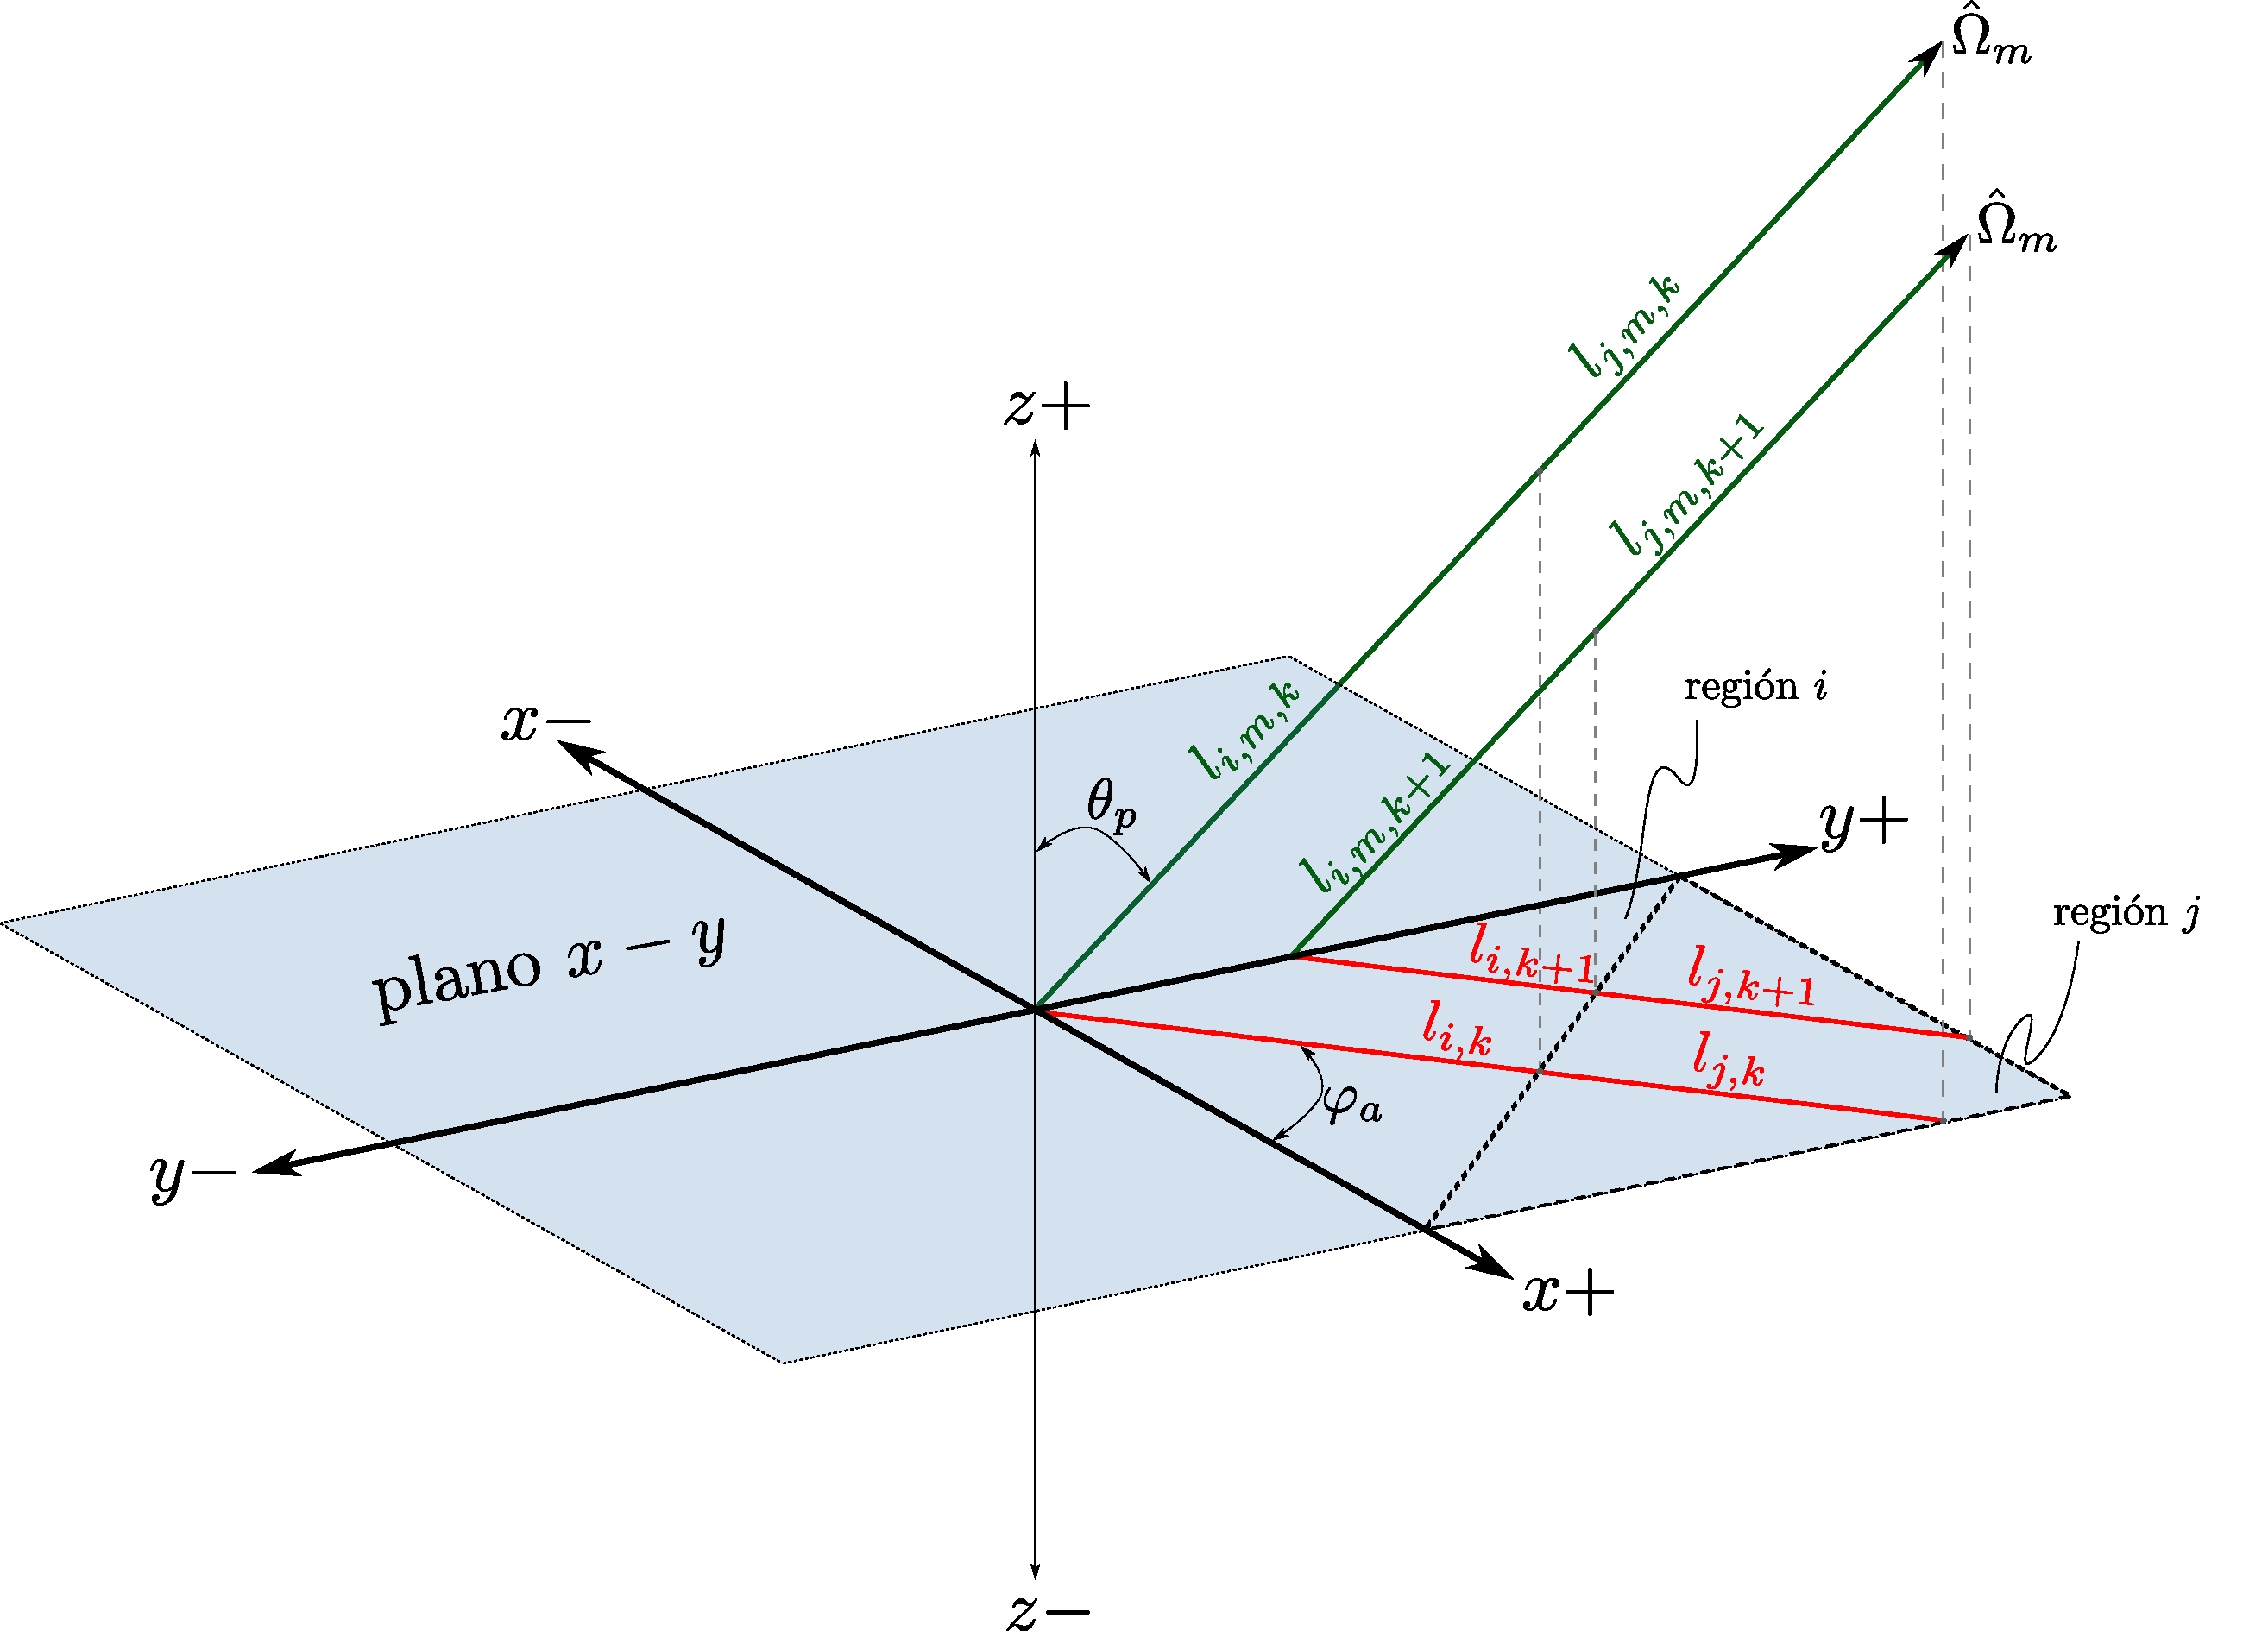
\includegraphics[width=1.0\linewidth]{coords-indices-2.pdf}
 \end{center}
\caption{\label{fig:coords-indices} Discretización espacial de la formulación MOC.}
\end{figure}

Por otra parte, las secciones eficaces responden a la nomenclatura usual:

\begin{itemize}
\renewcommand\labelitemi{$\cdot$}
 \item $\Sigma^s_{g^\prime \rightarrow g}$: sección eficaz de \emph{scattering} de grupo $g^\prime$ a $g$;
 \item $\Sigma^t_g$: sección eficaz total de grupo $g$;
 \item $\Sigma^f_g$: sección eficaz de fisión de grupo $g$; y
 \item $\nu$: número de neutrones por fisión.
\end{itemize}

Finalmente, se listan algunas definiciones usuales y otras específicas a MOC:

\begin{itemize}
\renewcommand\labelitemi{$\cdot$}
 \item $\psi^{\text{in}}_{i,g,m,k}$: flujo angular de entrada al segmento $k$ correspondiente a la región $i$, grupo $g$ y ángulo $\boldsymbol{\hat{\Omega}}_m$;
 \item $\psi^{\text{out}}_{i,g,m,k}$: flujo angular de salida del segmento $k$ correspondiente a la región $i$, grupo $g$ y ángulo $\boldsymbol{\hat{\Omega}}_m$;
 \item $\phi_{i,g}$: flujo escalar de la región $i$ y grupo $g$;
 \item $q_{i,g,m}$: fuente angular de la región $i$ y grupo $g$ con dirección $\hat{\Omega}_m$. Para \emph{scattering} isotrópico, $q_{i,g,m} = \frac{1}{4\pi}Q_{i,g}$, donde $Q_{i,g}$ es la fuente de la región $i$ y grupo $g$. De esta forma, $q_{i,g,m}$ es independiente del índice $m$, motivo por el cual se utiliza $q_{i,g,m} = q_{i,g}$.
 \item $l_{i,m,k}$: longitud del segmento $k$ con dirección angular $m$ dentro de la región $i$. Observando la figura~\ref{fig:coords-indices}, la igualdad $l_{i,m,k} = \frac{l_{i,k}}{\sin \theta_p}$ resulta obvia.
\end{itemize}

\subsection{Formulación de MOC}

La formulación multigrupo de la ecuación de transporte integro-diferencial estacionaria es~\cite{henry,lamarsh,duderstadt,glasstone,lewis,stammler,handbook-ingnuclear}

\begin{equation}
 \label{eq:transportemultigrupo}
 \boldsymbol{\hat{\Omega}} \cdot \text{grad} \left[ \psi_g(\vec{x}, \boldsymbol{\hat{\Omega}}) \right]
 + \Sigma^t_g(\vec{x}) \cdot \psi_g(\vec{x}, \boldsymbol{\hat{\Omega}}) = q_g(\vec{x}, \boldsymbol{\hat{\Omega}}),
\end{equation}

\noindent
donde, para el caso sin fuentes externas, el término de fuente posee las contribuciones de fisión (isotrópica) y \emph{scattering}

\begin{equation} \label{eq:fuentemultigrupo-1}
 q_g(\vec{x}, \boldsymbol{\hat{\Omega}}) =
 \sum_{g^\prime=1}^G \int_{4\pi} \Sigma^s_{g^\prime \rightarrow g}(\vec{x}, \boldsymbol{\hat{\Omega}^\prime} \rightarrow \boldsymbol{\hat{\Omega}}) \cdot \psi_{g^\prime}(\vec{x}, \boldsymbol{\hat{\Omega}^\prime}) \, d\boldsymbol{\hat{\Omega}^\prime} 
 + \frac{\chi_g}{4\pi k_{\text{eff}}} \sum_{g^\prime=1}^G \int_{4\pi} \nu\Sigma^f_{g^\prime}(\vec{x}) \cdot \psi_{g^\prime}(\vec{x}, \boldsymbol{\hat{\Omega}^\prime}) \, d\boldsymbol{\hat{\Omega}^\prime}.
\end{equation}

\noindent
Suponiendo \emph{scattering} isotrópico y utilizando la definición del flujo escalar a partir del flujo angular se pierde la dependencia con la dirección angular $\boldsymbol{\hat{\Omega}}$ y se obtiene

\begin{equation} \label{eq:fuentemultigrupo-2}
 q_g(\vec{x}, \boldsymbol{\hat{\Omega}}) = 
 q_g(\vec{x}) = 
 \frac{1}{4\pi} \left(
 \sum_{g^\prime=1}^G \Sigma^s_{g^\prime \rightarrow g}(\vec{x}) \cdot \phi_{g^\prime}(\vec{x})
 + \frac{\chi_g}{k_{\text{eff}}} \sum_{g^\prime=1}^G \nu\Sigma^f_{g^\prime}(\vec{x}) \cdot \phi_{g^\prime}(\vec{x}) 
 \right).
\end{equation}

Aplicando MOC a la ecuación de transporte multigrupo~\eqref{eq:transportemultigrupo} se obtiene una ecuación diferencial lineal de primer orden~\cite{glasstone,handbook-ingnuclear}

\begin{equation} \label{eq:caracteristica}
 \frac{d}{ds}\psi_g(\vec{r_0}+s\boldsymbol{\hat{\Omega}},\boldsymbol{\hat{\Omega}}) 
 + \Sigma^t_g(\vec{r_0}+s\boldsymbol{\hat{\Omega}}) \cdot \psi_g(\vec{r_0}+s\boldsymbol{\hat{\Omega}}, \boldsymbol{\hat{\Omega}}) = 
 q_g(\vec{r_0}+s\boldsymbol{\hat{\Omega}})
\end{equation}

\noindent
que será aplicada a cada segmento de cada \emph{track} trazado sobre la geometría a analizar. Estas líneas responden a la ecuación $\vec{r_0}+s\boldsymbol{\hat{\Omega}}$, donde $s$ es la distancia al punto $\vec{r_0}$ medida sobre la dirección $\boldsymbol{\hat{\Omega}}$. Como se verá a continuación, realizando un \emph{ray tracing} sobre la geometría del problema a partir de la selección de diferentes puntos de inicio $\vec{r_0}$ y direcciones $\boldsymbol{\hat{\Omega}}$ y resolviendo la ecuación característica~\eqref{eq:caracteristica} sobre cada uno de los segmentos de cada \emph{tracks}, es posible obtener la información necesaria para la determinación del flujo escalar en cada región y grupo de energía. Al discretizar la ecuación~\eqref{eq:caracteristica} y aplicar la notación descripta para este trabajo, se obtiene

\begin{equation} \label{eq:edo-disc}
 \frac{d}{ds}\psi_{i,g,m,k} (s)
 + \Sigma^t_{i,g} \cdot \psi_{i,g,m,k} (s) = 
 q_{i,g,m}
\end{equation}

\noindent
donde además se ha asumido la aproximación de fuente plana en cada región y por este motivo $q$ ha perdido la dependencia con $s$, resultando en

\begin{equation} \label{eq:fuente-isotropica}
 q_{i,g,m} = q_{i,g} = 
 \frac{1}{4\pi} \left(
 \sum_{g^\prime=1}^G \Sigma^s_{i,g^\prime \rightarrow g} \cdot \phi_{i,g^\prime}
 + \frac{\chi_g}{k_{\text{eff}}} \sum_{g^\prime=1}^G \nu\Sigma^f_{i,g^\prime} \cdot \phi_{i,g^\prime}
 \right).
\end{equation}

La ecuación~\eqref{eq:edo-disc} puede ser resuelta para cada segmento de cada \emph{track}, siempre y cuando se conozca la condici\'on inicial. En particular, el resultado para el flujo angular a la salida de un segmento es

\begin{equation}
 \psi^{\text{out}}_{i,g,m,k} = \psi^{\text{in}}_{i,g,m,k} \cdot e^{-\tau_{i,g,m,k}}
 + \frac{q_{i,g}}{\Sigma^t_{i,g}} \left(1 - e^{-\tau_{i,g,m,k}} \right),
\end{equation}

\noindent
siendo $\tau_{i,g,m,k}$ el camino óptico, definido como el producto $l_{i,m,k} \cdot \Sigma^t_{i,g}$. Reacomodando, la variación del flujo angular en un segmento puede escribirse como

\begin{equation} \label{eq:delta-psi}
 \Delta \psi_{i,g,m,k} = 
 \psi^{\text{in}}_{i,g,m,k} - \psi^{\text{out}}_{i,g,m,k} = 
 \left( \psi^{\text{in}}_{i,g,m,k} - \frac{q_{i,g}}{\Sigma^t_{i,g}} \right) \left(1 - e^{-\tau_{i,g,m,k}} \right).
\end{equation}

El valor medio del flujo angular del segmento $k$ correspondiente a la región $i$, grupo $g$ y dirección polar $p$ se obtiene integrando la soluci\'on de la ecuación~\eqref{eq:edo-disc} de la siguiente forma

\begin{multline}
 \overline{\psi}_{i,g,m,k} =
 \frac{1}{l_{i,m,k}} \int_{s_{\text{in}}}^{s_{\text{out}}} \psi_{i,g,m,k} (s) \, ds = \\
 \frac{1}{l_{i,m,k}} \left[ \frac{\psi^{\text{in}}_{i,g,m,k}}{\Sigma^t_{i,g}} \left(1 - e^{-\tau_{i,g,m,k}} \right) + \frac{l_{i,m,k} \cdot q_{i,g}}{\Sigma^t_{i,g}} \left( 1 - \frac{\left(1 - e^{-\tau_{i,g,m,k}} \right)}{\tau_{i,g,m,k}} \right) \right].
\end{multline}

\noindent
Luego, utilizando el resultado de la ecuación~\eqref{eq:delta-psi} sobre la expresi\'on del flujo angular medio, se obtiene

\begin{equation} \label{eq:flujo-ang-medio-en-segmento}
 \overline{\psi}_{i,g,m,k} = \frac{q_{i,g}}{\Sigma^t_{i,g}} + \frac{\Delta \psi_{i,g,m,k}}{\tau_{i,g,m,k}}.
\end{equation}

El flujo angular medio en la región $i$, grupo $g$ y ángulo $\boldsymbol{\hat{\Omega}}_m$ puede ser obtenido a partir de la contribuci\'on de cada segmento $k$ en la región $i$

\begin{equation} \label{eq:flujo-ang-medio-en-region}
 \overline{\psi}_{i,g,m} = \frac{\sum_{k(i,m)} \overline{\psi}_{i,g,m,k} l_{i,k} \delta_m}{\sum_{k(i,m)} l_{i,k} \delta_m},
\end{equation}

\noindent
donde $k(i,m)$ representa los segmentos correspondientes a una región $i$ con dirección $\boldsymbol{\hat{\Omega}}_m$ y $\delta_m$ la separaci\'on entre segmentos para un dado ángulo azimutal especificado en $\boldsymbol{\hat{\Omega}}_m$. Para encontrar al flujo escalar en una región $i$ y a un grupo $g$, basta con integrar en ángulo s\'olido la expresi\'on obtenida en~\eqref{eq:flujo-ang-medio-en-region} de la siguiente manera

\begin{equation} \label{eq:flujo-escalar-1}
 \phi_{i,g} = \int_{4\pi} \overline{\psi}_{i,g} (\boldsymbol{\hat{\Omega}}) \, d\boldsymbol{\hat{\Omega}} \approx 
 4\pi \sum_m w_m \overline{\psi}_{i,g,m}.
\end{equation}

\noindent
En este caso, $w_m$ son los pesos de la cuadratura angular normalizados, de forma que $\sum_m w_m = \sum_a \sum_p w_a w_p = \sum_a w_a \sum_p w_p = 1$. En primera instancia, es necesario implementar el resultado obtenido en la ecuación~\eqref{eq:flujo-ang-medio-en-region} en~\eqref{eq:flujo-escalar-1}

\begin{equation} \label{eq:flujo-escalar-2}
 \phi_{i,g} =
 4\pi \sum_m \left( w_m \frac{\sum_{k(i,m)} \overline{\psi}_{i,g,m,k} l_{i,k} \delta_m}{\sum_{k(i,m)} l_{i,k} \delta_m} \right) = 
 \frac{4\pi}{A_i} \sum_m \left( w_m \delta_m \sum_{k(i,m)} \overline{\psi}_{i,g,m,k} l_{i,k} \right).
\end{equation}

\noindent
En la anterior ecuación puede verse que el t\'ermino $A_{i,m} = \sum_{k(i,m)} l_{i,k} \delta_m = \delta_m \sum_{k(i,m)} l_{i,k}$ representa el área de la región $i$ computada a partir de los segmentos $l_{i,k}$ (proyectados sobre el plano $x - y$) y con ángulo azimutal contenido en $\boldsymbol{\hat{\Omega}}_m$. En un \emph{ray tracing} con la suficiente densidad de lineas puede suponerse que el área obtenida a partir de esta expresi\'on es independiente de la dirección azimutal de los segmentos, motivo por el cual $A_{i,m} = A_i$ y es retirado de la sumatoria sobre $m$.

Por último, la expresi\'on para el flujo escalar puede simplificarse aún m\'as incorporando el resultado de la ecuación~\eqref{eq:flujo-ang-medio-en-segmento} sobre~\eqref{eq:flujo-escalar-2}

\begin{multline} \label{eq:flujo-escalar-3}
 \phi_{i,g} =
 \frac{4\pi}{A_i} \sum_m \left\lbrace w_m \delta_m \sum_{k(i,m)} \left[ l_{i,k} \left( \frac{q_{i,g}}{\Sigma^t_{i,g}} + \frac{\Delta \psi_{i,g,m,k}}{\tau_{i,g,m,k}} \right) \right] \right\rbrace \\ 
 = \frac{4\pi}{A_i} \cdot \frac{q_{i,g}}{\Sigma^t_{i,g}} \sum_m \left( w_m \delta_m \sum_{k(i,m)} l_{i,k} \right) + \frac{4\pi}{A_i \cdot \Sigma^t_{i,g}} \sum_m \left( w_m \delta_m \sin \theta_p \sum_{k(i,m)} \Delta \psi_{i,g,m,k} \right) \\ 
 = \frac{4\pi}{\Sigma^t_{i,g}} \left[ q_{i,g} + \frac{1}{A_i} \sum_m \left( w_m \delta_m \sin \theta_p \sum_{k(i,m)} \Delta \psi_{i,g,m,k} \right) \right]
 .
\end{multline}

La resolución de las ecuaciones~\eqref{eq:fuente-isotropica}, \eqref{eq:delta-psi} y~\eqref{eq:flujo-escalar-3} permiten obtener la distribución espacial y energética del flujo escalar. Sin embargo, el proceso es iterativo hasta que los criterios de convergencia del flujo, fuentes, condiciones de contorno y valor de $k_{\text{eff}}$ sean satisfechos. Comúnmente, el nombre atribuido a cada una de estas iteraciones se conoce como \emph{transport sweep}. En cada \emph{transport sweep} se calcula el flujo escalar con~\eqref{eq:flujo-escalar-3} a partir de las contribuciones del flujo angular sobre cada región y grupo obtenidas mediante~\eqref{eq:delta-psi}. Posteriormente se computa el factor de multiplicación y se actualizan los valores de las fuentes $q_{i,g}$ seg\'un \eqref{eq:fuente-isotropica}.

{\color{red}Falta hablar de las cuadraturas cuadraturas}

\section{Geometr\'ias en milonga}

Las geometrias en milonga se interpretan a traves de mallas, ya sean estructuradas o no estructuradas. 

caso particular de moc: tienen que ser un dominio rectangular, pero oprque es así lo explico mas adelante.

\subsection{Mallas estructuradas y no estructuradas}

\subsection{\emph{Ray tracing} de mallas 2D}

La realizaci\'on del \emph{ray tracing} sobre la geometría del problema a resolver es uno de los pasos más importantes que debe afrontarse en el método de las características. Luego de este procedimiento, se dispone de las estructuras de datos que almacenan información de los \emph{tracks}, principalmente los segmentos que los forman y la región a la que cada uno de ellos pertenece. Como se ha visto anteriormente, la actual formulación MOC implementada en milonga acepta únicamente dominios rectangulares. El motivo de esta limitación radica en que el tipo de algoritmo de \emph{ray tracing} desarrollado es de tipo c\'iclico. 

Por simetr\'ia, solo es necesario trazar \emph{tracks} con $\varphi \in \left[ 0, \pi \right]$ debido a que aquellos con $\varphi + \pi$ poseen los mismos puntos de definición. Por otro lado, los \emph{tracks} con ángulos azimutales suplementarios tiene un espaciado tal que forman recorridos cerrados. 

mostramos un ejemplo de figura de tracks ciclicos

especificamos que tipo de mallas podemos trackear (elementos de cualquier tipo)

checkeamos los volumenes frente a los verdaderos (es opcional)

comentamos que si se supera tal tau, los segmentos los cortamos

dependiendo de la condicion de contorno, los tracks ciclicos se unen de diferentes formas


\subsection{Discusi\'on acerca de geometr\'ias}

se deberia hacer un modulo mas eficiente para cargar geometrias.

\section{MOC solver}
aca hacemos un grafico tambien de como recorremos los rayos en una masha

\section{Input}

\section{Resultados}

\section{Conclusiones}

\label{lastpage}

\printbibliography

\end{document}

